

\section{Klasse Calendar} 

Die Klasse \emph{Calendar} ist ein zentrales Element der Anwendungslogik der Webanwendung.
Hier befinden sich Methoden zur Berechnung und Auswahl eines Datums oder Zeitraums,
von denen so gut wie die gesamte Softwarefunktionalit\"at abh\"angig ist.
Dazu geh\"oren zum Beispiel das Zeichnen des Graphen oder das Anfragen von Patienteninformationen 
f\"ur einen ausgew\"ahlten Zeitabschnitt der Therapie.
Die Abbildung 5.1 zeigt das \emph{Calendar-Widget} der Websoftware.
Dieses Widget wird in der \emph{Calendar}-Klasse berechnet.
Nach der Berechnung werden die Daten zum Anzeigen in der Pr\"asentationsschicht weitergegeben.\\

\begin{figure}[h]
  \centering
  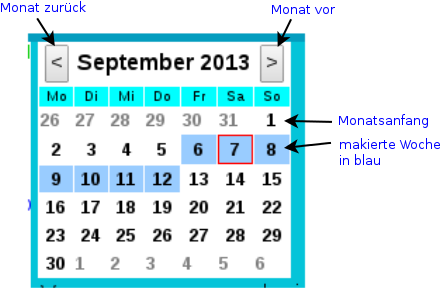
\includegraphics[scale=0.7]{screenshots/kapitel5/calendar_widget_beschriftet.png}
  \caption{Calendar-Widget}
  
\end{figure}

In der Klasse Calendar sind folgende Klassen-Member enthalten:
\begin{itemize}
 \item calendarResolutionModif:\\
 Dieses Element wurde bereits erl\"autert. Es ist ein Modifikator f\"ur die Aufl\"osung der Zeitachse.
 
 \item currentDate:\\
 Hier wird das aktuelle Datum hinterlegt. 
 
 \item viewedMonthStart:\\
 In dieser Variablen ist ein Datum-Objekt f\"ur den angezeigten Monatsanfang hinterlegt.
 Der Monatsanfang soll immer griffbereit sein.
 Er ist notwendig f\"ur die Berechnung der richtigen Zelle im Kalender, in der ein Tag eingetragen wird.
 In der Abbildung 5.1 ist zu sehen,
 dass der erste Tag des angezeigten Monats September, ein Sonntag ist.
 Er taucht nicht in der ersten, sondern in der letzten Zelle im Kalender auf.
 Davor und am Ende des Monats werden die Zellen grau ausgef\"ullt und nummeriert.
 F\"ur diese Kalkulationen ist die Variable \emph{viewedMonthStart} besonders wichtig.
 
 \item markedDate:\\
 Je nach Zeitachsenaufl\"osung wird ein Tag, eine Woche oder der Monat selbst als markiert gew\"ahlt.
 Die Variable \emph{markedDate} speichert den markierten Tag.
 Der Hintergrund eines markierten Tages wird ebenfalls, wie in der markierten Woche zu sehen ist, 
 blau gef\"ullt.
 
 \item markedWeek:\\
 Die Variable \emph{markedWeek} ist ein Array und speichert insgesamt sieben Zellen.
 Diese Zellen repr\"asentieren eine markierte Woche.
 Im Widget werden diese Zellen anschlie\ss{}end blau gezeichnet.
 
 \item drawMatrix:\\
 Das zweidimensionale Array \emph{drawMatrix} speichert pro Zelle eine Datenstruktur.
 Die Elemente der Datenstruktur beinhalten Informationen 
 wie die Zelle in der Pr\"asentationsschicht gezeichnet werden soll.
 Hier werden folgende Informationen f\"ur je eine Zelle des Kalenders hinterlegt:\\
 \emph{DAY\texttt{\_}NUMBER}: Zahl f\"ur den Tag im Kalender.\\
 \emph{ONMONTH}: Sagt aus, ob die Zelle sich im aktuellen Monat (schwarz beschriftet) oder 
 au\ss{}erhalb des Monats (grau beschriftet) befindet.\\
 \emph{DATUM}: Hier wird ein vollst\"andiges Datumsobjekt f\"ur diese Zelle hinterlegt.\\
 \emph{HIGHLITE}: Diese Variable ist f\"ur eine zuk\"unftige Funktionalit\"at des Kalenders reserviert.\\
 \emph{CURRENT\texttt{\_}DAY}: Das Flag sagt aus, ob das Datum der Zelle dem aktuellen Tag entspricht.\\
 \emph{MARKED}: Dieses Flag sagt aus, ob die Zelle markiert ist.\\
 
\end{itemize}

Abgesehen von der internen Logik, bietet die Klasse \emph{Calendar}, Methoden f\"ur die Webanwendung an
und l\"asst sich so durch den Benutzer kontrollieren.

\begin{itemize}


 \item recalculate:\\
 Die Methode \emph{recalculate()} wird automatisch gerufen, 
 wenn eine \"Anderung durch den Benutzer am Kalender erfolgt.
 Wird zum Beispiel zum n\"achsten Monat gewechselt, 
 so wird die \emph{drawMatrix} neu berechnet und kann neu gezeichnet werden.
 \item nextMonth, prevMonth:\\
 Der Wechsel zum n\"achsten oder zum vorherigen Monat wird \"uber die Methoden \emph{nextMont()} 
 und \emph{prevMont()} gemacht.
 \item resolutionModif:\\
 Hat der Benutzer die Aufl\"osung von Woche auf Tag oder Monat umgestellt, 
 so wird das intern \"uber die Methode \emph{resolutionModif()} ausgef\"uhrt.
 \item jumpToCurrentDay:\\
 Die Methode \emph{jumpToCurrentDay()} erlaubt dem System nach Interaktion des Benutzers zum aktuellen Tag, 
 Monat oder zur aktuellen Woche zu springen.
 \item prevDay, nextDay:\\
 Der Benutzer hat auch die M\"oglichkeit in der Graphen- und Mahlzeitenansicht 
 mit der Intervalll\"ange von einem Tag vor oder zur\"uck zu gehen.
 Das wird intern \"uber die Methoden \emph{nextDay()} und \emph{prevDay()} getan.
\end{itemize}